\documentclass[fleqn, 10pt]{beamer}


\title{\LaTeX{} Training}
\author[J. Fogel]{Jamie Fogel \\
        Research Assistant \\
        Federal Reserve Bank of Boston \\
        \href{mailto:james.fogel@bos.frb.org}{james.fogel@bos.frb.org}
        }
\date[August 2013]{August 1, 2013}

\def\tex{S:/trainings/stata/tex}
\def\results{S:/trainings/LaTeX/results}
\def\graph_{G:/Deptdata/Research/Share/RE-RKT-A/directors_apr_2013/results}

\usetheme{AnnArbor}
\usecolortheme{wolverine}

\setbeamertemplate{footline}
{%
  \begin{beamercolorbox}{section in head/foot}
	\hspace{1em} \insertshortauthor \hfill \inserttitle , \insertshortdate \hfill \insertframenumber /  \inserttotalframenumber \hspace{1em}
  \end{beamercolorbox}%
}




\usepackage{hyperref}
\usepackage{import}
\usepackage{caption}
\captionsetup{labelformat=empty,labelsep=none}
\usepackage{amsmath}
\setlength{\mathindent}{0.5 em}
\usepackage{wrapfig}
\usepackage{comment}
\usepackage{listings}
\usepackage{booktabs}
\usepackage{longtable}
\usepackage{setspace}
%\usepackage{doc}
%\usepackage[caption=false]{subfig}


\usebeamercolor{structure}
\usebeamercolor{frametitle}
%\setbeamercolor{block title}{bg=\color{structure.fg}, fg=black}

\lstset{basicstyle= \ttfamily \scriptsize, frame=trbl, backgroundcolor=\color{frametitle.bg},rulecolor=\color{structure.fg}}
\usepackage{xcolor}

\def\lst{\lstinline}

\newcommand{\com}[1]{{\footnotesize\texttt{#1}}}

\hypersetup{
    bookmarks=true,                 % show bookmarks bar?
    unicode=false,                  % non-Latin characters in bookmarks
    pdftoolbar=true,                % show toolbar?
    pdfmenubar=true,                % show menu?
    pdffitwindow=true,              % window fit to page when opened
    pdfstartview={FitH},            % fits the width of the page to the window
    pdftitle={},                    % title
    pdfauthor={Jamie Fogel},        % author
    pdfnewwindow=true,              % links in new window
    colorlinks=true,                % false: boxed links; true: colored links
    linkcolor=blue,                 % color of internal links
    citecolor=black,                % color of links to bibliography
    filecolor=magenta,              % color of file links
    urlcolor=blue,                  % color of external links
    breaklinks=true
}


\begin{document}


\begin{frame}[plain]
    \titlepage
\end{frame}

\section{Introduction}

\begin{frame}{What is \LaTeX{}?}
    \begin{itemize}
        \item\LaTeX{} is a typesetting language --- not only does it contain your text, it also contains commands which specify how your document will look. These commands give instructions like ``start a new section here,'' ``include a figure using a specified image file here,'' or ``put a footnote here.''
        \item It is a substitute for word processors like Microsoft Word; it allows for much more control over your document but has higher startup costs
    \end{itemize}
\end{frame}

\begin{frame}{Why/when should you use \LaTeX{}}
    \begin{itemize}
        \item \LaTeX{} allows you a great deal of control over your document \pause
        \item \LaTeX{} has much better equation, graphics, and table capabilities than Word \pause
        \item \LaTeX{} interacts well with Stata \pause
        \item \LaTeX{} allows you to automate your citations and references section \pause
        \item \LaTeX{} is widely used in academia; your grad school resume should probably be in \LaTeX{}! \pause
        \item Unfortunately, startup costs are higher in \LaTeX{} than in WYSIWYG word processors like Word; if all you want is a simple text document or if you need to finish very quickly you might be better off using Word
    \end{itemize}
\end{frame}


\begin{frame}{Disclaimer}
    \textbf{Disclaimer: my terminology may be imperfect or imprecise here so feel free to correct me. I am simply using these phrases as I have come to understand and use them at the Boston Fed.}
\end{frame}


\begin{frame}{Different versions of \LaTeX{}}

    There are three versions of \LaTeX{} to be familiar with: \pause
    \begin{enumerate}
        \item \LaTeX{} --- the traditional version. You will use \LaTeX{} for creating documents analogous to what you might create with a word processor. \pause
        \item Beamer --- the presentation version of \LaTeX{}. Beamer presentations are analogous to Powerpoint presentations; this presentation is written in Beamer. Beamer is nearly identical to \LaTeX{} code; the primary differences are that to create a Beamer presentation you declare the document class to be ``beamer'' in the document's preamble (described soon) and the document is organized into separate frames (slides). \pause
        \item BibTeX --- BibTeX is a special package for automating citations that is compatible with both \LaTeX{} and Beamer. \pause
    \end{enumerate}
    This presentation will focus on creating simple \LaTeX{} documents, however it is simple to start writing Beamer documents once you have a basic understanding of \LaTeX{}.
\end{frame}

\begin{frame}{The .tex file}
    \begin{itemize}
        \item All \LaTeX{} code is written in a .tex file. This file is analogous to a do-file in Stata or a .m-file in MATLAB.
        \item Your .tex file may reference external files, such as other .tex files or image files, but it is the backbone (and often the entire body) of your document.
        \item Once you have created your .tex file, you ``compile'' it into a PDF. The .tex file is just a bunch of code, however the compiled PDF will be a presentation-quality finished product.
    \end{itemize}
\end{frame}

\section{Basic Elements of a \LaTeX{} Document}

\begin{frame}[fragile]{\LaTeX{} Document Structure}
    A .tex file is divided into two sections: the preamble and the document text.
    \begin{enumerate}
        \item Preamble --- The preamble is where you load packages of \LaTeX{} features (basically you are telling \LaTeX{} which toolboxes you want to use) and define certain parameters which govern how the document will look. For example, you could choose a font, define color schemes, or design headers and footers. The parameters you define in the preamble apply to your entire document, although they can be overridden.
        \item Document text --- The ``document text'' is where you include all of your text, tables, figures, and any code that does not define how the entire document will look. All of the code in the ``document text'' section follows the command \lst=\begin{document}= and precedes the last line of the .tex file, \lst=\end{document}=. You will spend almost all of your time working on the document text part of the .tex file.
    \end{enumerate}
\end{frame}

\subsection{Preamble}

\begin{frame}[fragile]{Preamble}
    When I start a new .tex file, rather than writing my preamble from scratch, I usually just copy the preamble from an existing document and make adjustments as necessary. This works because there is typically not a lot of variation in what I want to include in the preamble.

    To get started, I suggest you copy the preamble from one of my documents.
    \begin{itemize}
        \item For a \LaTeX{} document, use the preamble from the \LaTeX{} template accompanying this presentation.
        \item For a Beamer presentation, use the preamble from this document.
    \end{itemize}
\end{frame}

\begin{frame}[fragile]{Sample preamble code}
    \begin{lstlisting}
% Open document
\documentclass[11pt]{article}

% Loading packages
\usepackage[margin=1in]{geometry}
\usepackage{amsmath}
\usepackage{hyperref}
\usepackage{natbib}
\usepackage{subfig}

% Define how hyperlinks will look
\hypersetup{
    colorlinks=true,                % false: boxed links; true: colored links
    linkcolor=blue,                 % color of internal links
    citecolor=black,                % color of links to bibliography
    urlcolor=blue,                  % color of external links
}
% Define a macro ``results'' to hold the filepath for Stata output
\def\results{S:/trainings/LaTeX/results}

\title{\LaTeX{} Training}
\author{Jamie Fogel}

\begin{document}
...
\end{document}
    \end{lstlisting}
\end{frame}

\subsection{Document Text}

\begin{frame}[fragile]{Document text}
    The document text is the meat of your \LaTeX{} document. In it you will type the text of your document, create tables and figures, and just about everything else. The rest of this presentation will primarily focus on the document text.
    \begin{lstlisting}
% Open document
\documentclass[11pt]{article}

...
% Preamble
...

\begin{document}

\maketitle

This is my sample \LaTeX{} document. Maybe I will write an equation: $e=mc^2$.

I could also create a simple table:

\begin{tabular}{ccc}
 1 & 2 & 3 \\
 4 & 5 & 6 \\
 7 & 8 & 9 \\
\end{tabular}

\end{document}
    \end{lstlisting}
\end{frame}


\subsection{Commands}

\begin{frame}[fragile]{Commands}
    Commands are one of the basic building blocks of \LaTeX{} code. Most commands begin with a backslash (\textbackslash) and can take arguments in either square braces ([]) or curly braces(\{\}). Commands perform tasks such as changing the font size, inserting a citation, caption or footnote, or changing the alignment of text.

    \begin{lstlisting}
\textbf{This text will be bold}
\section{Section title for new section created by this command}

% This command creates a row in a table that spans multiple columns
\multicolumn

% This command inserts an image file into your document
\includegraphics[width=10cm]{filepath.eps}

% Insert a title page, using inputs from the commands \title{} and \author{}
\maketitle
    \end{lstlisting}
\end{frame}

\subsection{Symbols}

\begin{frame}[fragile]{Symbols}
    \LaTeX{} symbols include virtually anything you will ever need when typing equations --- operators, Greek letters, fractions, powers, indices, and many more --- and are quite easy to use. They generally are written in the form \lst=\symbolname=. There is a learning curve, as it takes time to remember symbol names, however names are usually intuitive and you will pick up on them quickly. In order to use most mathematical symbols you must use the \lst=amsmath= package by including the line \lst=\usepackage{amsmath}= in your preamble.
    \begin{columns}
        \column{.68\textwidth}
    \begin{lstlisting}
$\forall x \in X, \quad \exists y \leq \epsilon$ \\
$\cos (2\theta) = \cos^2 \theta - \sin^2 \theta$ \\
$\lim_{x \to \infty} \exp(-x) = 0 $ \\
$k_{n+1} = n^2 + k_n^2 - k_{n-1} $ \\
$\frac{n!}{k!(n-k)!} = {n \choose k } $ \\
    \end{lstlisting}
        \column{.3\textwidth}
            {\scriptsize
                $\forall x \in X, \quad \exists y \leq \epsilon $ \\ \vspace{.2cm}
                $\cos (2\theta) = \cos^2 \theta - \sin^2 \theta $ \\ \vspace{.2cm}
                $\lim_{x \to \infty} \exp(-x) = 0 $ \\ \vspace{.2cm}
                $k_{n+1} = n^2 + k_n^2 - k_{n-1} $ \\ \vspace{.2cm}
                $\frac{n!}{k!(n-k)!} = {n \choose k } $ \\
            }
    \end{columns}
\end{frame}

\subsection{Environments}

\begin{frame}[fragile]{Symbols}
    A \LaTeX{} environment is composed of two commands: \lst=\begin{environmentname}= and \lst=\end{environementname}=. Environments define a set of actions to be taken upon everything within the environment. For example, the \lst=tabular= environment knows that all of the text inside it defines a table and typesets it appropriately. Other commonly-used environments include \lst=figure=, \lst=align= (for nicely-formatted equations), \lst=itemize=, \lst=enumerate=, and \lst=theorem=.
\end{frame}

\begin{frame}[fragile]
 \begin{columns}[T]
        \column{.45\linewidth}
            \begin{lstlisting}
\begin{enumerate}
    \item First item
    \item Secon item
\end{enumerate}

\begin{itemize}
    \item First item
    \item Secon item
\end{itemize}

\begin{tabular}{ccc}
 1 & 2 & 3 \\
 4 & 5 & 6 \\
 7 & 8 & 9 \\
 \end{tabular}
            \end{lstlisting}
        \column{.45\linewidth}
 Enumerate environment
\begin{enumerate}
    \item First item
    \item Second item
\end{enumerate}

Itemize environment
\begin{itemize}
    \item First item
    \item Second item
\end{itemize}

Tabular environment \\
\begin{tabular}{ccc}
 1 & 2 & 3 \\
 4 & 5 & 6 \\
 7 & 8 & 9 \\
\end{tabular}
    \end{columns}
\end{frame}

\section{Equations}

\begin{frame}{Introduction to equations}
    If you have ever tried to insert equations in a word processor, you know that it can be a total mess. Not only is it difficult to make the equations look exactly the way you would like them to, if you try to do anything complicated like numbering your equations, the whole process can quickly devolve into chaos. Fortunately, \LaTeX{} provides a number of tools for including equations in a document.
\end{frame}

\begin{frame}[fragile]{Math environments}
    There are two ways of displaying equations/mathematical elements in \LaTeX{}:
    \begin{enumerate}
        \item text --- equations are displayed within the body of text where they are declared. For example, $y=x\beta+\epsilon$.
        \item displayed --- equations are separate from the main body of text. For example,
            \begin{align}
                y&=x\beta+\epsilon
            \end{align}
    \end{enumerate}
    In order to use mathematical expressions, you must open an environment that allows math. There are a number of possible environments which will all do the trick in similar ways; in this presentation I will focus on two --- the \lst=math= environment for in text equations, and the \lst=align= environment for display equations.
\end{frame}

\subsection{The Math Environment}
\begin{frame}[fragile]{The Math Environment}
    The \lst=math= environment is suitable for including bits of math or equations within your text. The \lst=math= environment is opened and closed by dollar signs (\$). If you forget the dollar sign you will get an error message, often including the phrase ``undefined control sequence.''

    \begin{lstlisting}
Here is a simple in-text equation using the math environment:
    $\sin^2 \theta + \cos^2 \theta = 1$
    \end{lstlisting}
Here is a simple in-text equation using the math environment: $\sin^2 \theta + \cos^2 \theta = 1$
\end{frame}

\subsection{The Align Environment}

\begin{frame}[fragile]{The Align Environment}
    The \lst=align= environment creates publication-quality displayed equations. The \& tells \LaTeX{} to align the equals signs in all equations.
    \begin{lstlisting}
\begin{align}
    \tilde{E} &= \bar{e}(E+U+N)\\
    \tilde{U} &= \frac{\bar{e}\bar{u}(E+U+N)}{1-\bar{u}}\\
    \tilde{N} &= (E+U+N)(1-\bar{e}-\frac{\bar{e}\bar{u}}{1-\bar{u}})
\end{align}
    \end{lstlisting}
    \pause
{\scriptsize
    \begin{align}
        \tilde{E} &= \bar{e}(E+U+N)\\
        \tilde{U} &= \frac{\bar{e}\bar{u}(E+U+N)}{1-\bar{u}}\\
        \tilde{N} &= (E+U+N)(1-\bar{e}-\frac{\bar{e}\bar{u}}{1-\bar{u}})
    \end{align}
}
\end{frame}

\begin{frame}[fragile]{The Align Environment --- No Equation Numbers}
Now, suppose we want to omit the equation numbers. We do this by replacing ``align'' with ``align*'', shown below:
    \begin{lstlisting}
\begin{align*}
    \tilde{E} &= \bar{e}(E+U+N)\\
    \tilde{U} &= \frac{\bar{e}\bar{u}(E+U+N)}{1-\bar{u}}\\
    \tilde{N} &= (E+U+N)(1-\bar{e}-\frac{\bar{e}\bar{u}}{1-\bar{u}})
\end{align*}
    \end{lstlisting}
\pause
{\scriptsize
    \begin{align*}
        \tilde{E} &= \bar{e}(E+U+N)\\
        \tilde{U} &= \frac{\bar{e}\bar{u}(E+U+N)}{1-\bar{u}}\\
        \tilde{N} &= (E+U+N)(1-\bar{e}-\frac{\bar{e}\bar{u}}{1-\bar{u}})
    \end{align*}
}
\end{frame}

\section{Figures}


\begin{frame}[fragile]{A simple example}
In \LaTeX{} figures are created using the \lst=figure= environment. \\

Let's begin by creating a very simple figure. In Stata, I plotted labor force flows from employed to unemployed in eps format and saved it as ``S:/trainings/LaTeX/results/EE.eps.'' If all we want is a very simple figure, we simply tell \LaTeX{} to open the \lst=figure= environment, reference the saved image file we want to include in the figure, and finally close the \lst=figure= environment. The code on the left produces the figure on the right. \pause

\begin{figure}[h!]
    \begin{minipage}[c]{.5\textwidth}
        \centering
        \begin{lstlisting}
\begin{figure}[h!]
   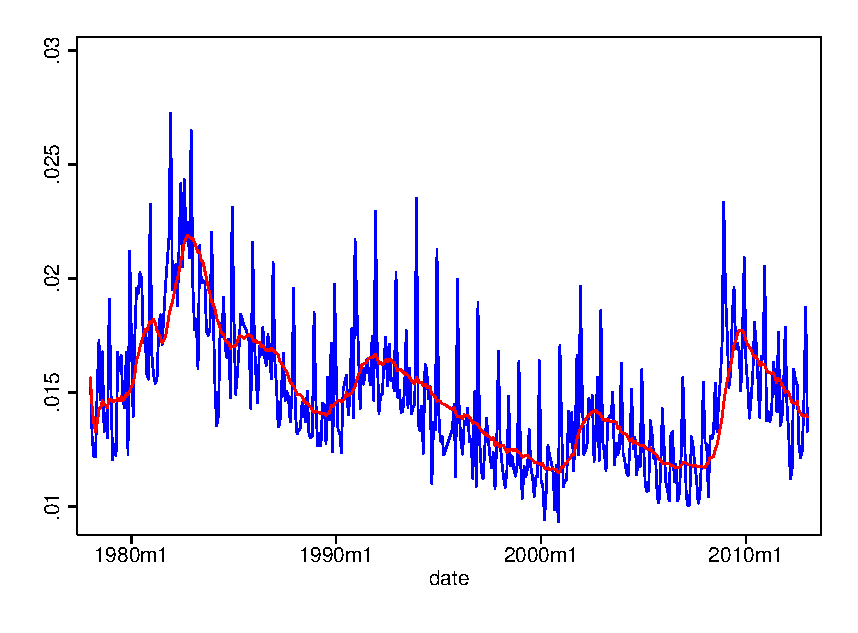
\includegraphics{\results/EU.eps}
\end{figure}
        \end{lstlisting}
    \end{minipage} \pause
    \begin{minipage}[c]{.45\textwidth}
        \centering
        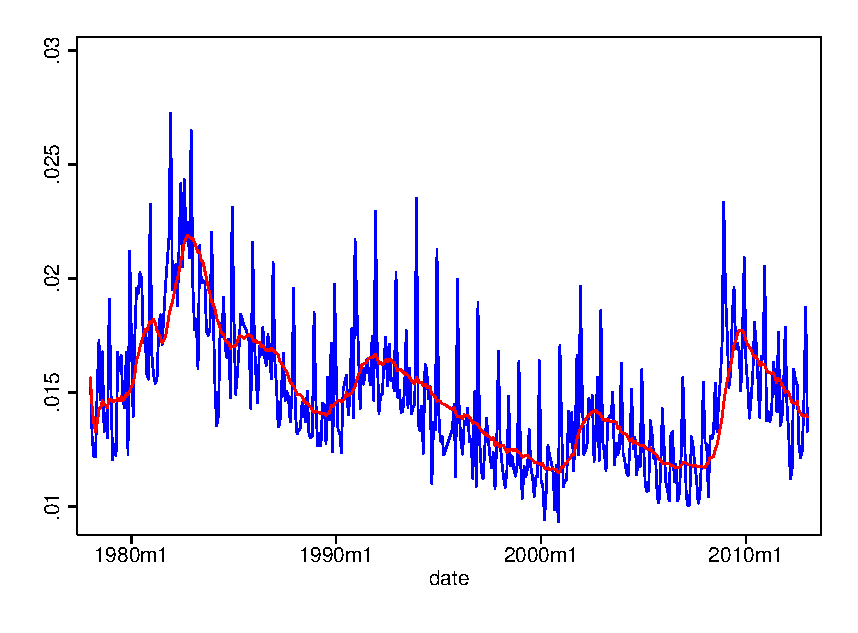
\includegraphics[width=.95\textwidth]{\results/EU.eps}
    \end{minipage}
\end{figure}
\end{frame}

\begin{frame}[fragile]{A more complicated example}
    The preceding figure was very plain; most figures include at least a caption and footnote.
    \begin{lstlisting}
    \begin{figure}[h!]
        \centering
        \caption{Employed to Unemployed Flows}
        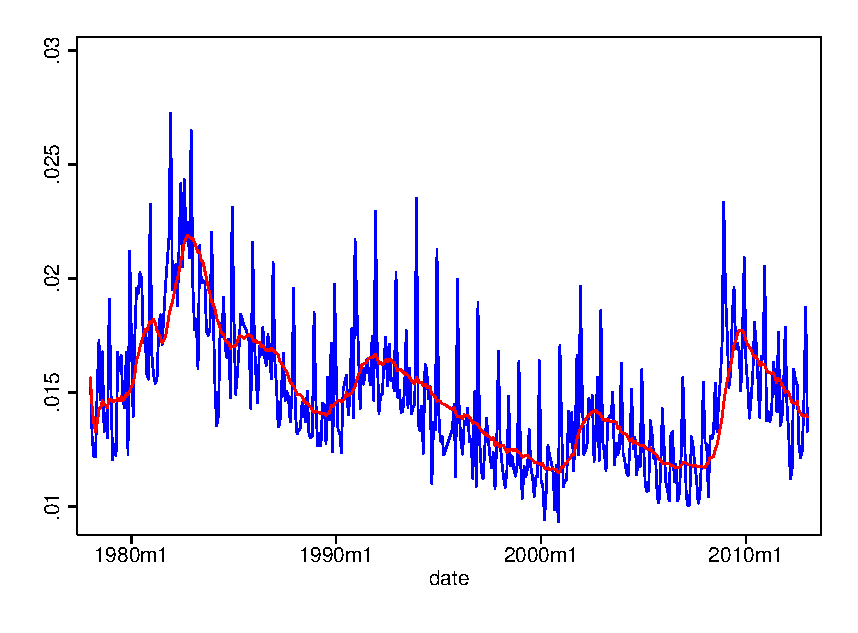
\includegraphics[width=.45\textwidth]{\results/EU.eps}\\
        \flushleft \footnotesize Flows in blue; 12-month moving average in red.\\ Source: BLS and Author's Calculations
    \end{figure}
    \end{lstlisting}
    \vspace{-.5cm}
    \begin{figure}[h!]
            \centering
            \caption{\scriptsize Employed to Unemployed Flows}
            \vspace{-.25cm}
            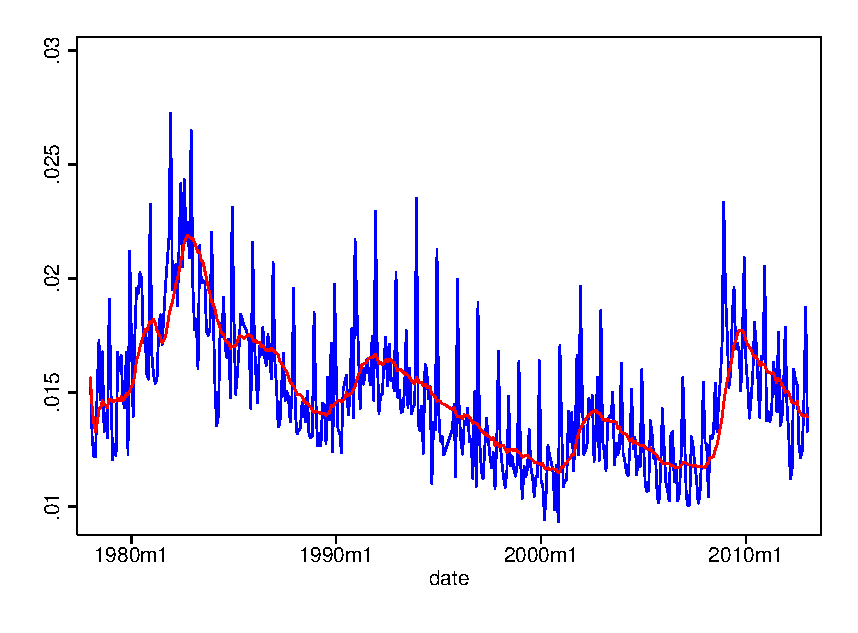
\includegraphics[width=.45\textwidth]{\results/EU.eps}\\
            \vspace{-.25cm}
            \scriptsize Flows in blue; 12-month moving average in red. Source: BLS and Author's Calculations
    \end{figure}
\end{frame}


\begin{frame}[fragile]{Combining multiple figures in \LaTeX{}}
    In \LaTeX{} it is possible to combine multiple figures and give each subfigure its own caption using the \lst=subfig= package
    \begin{lstlisting}
\begin{figure}
    \caption{Labor Force Flows}
    \centering
    \subfloat[EE]{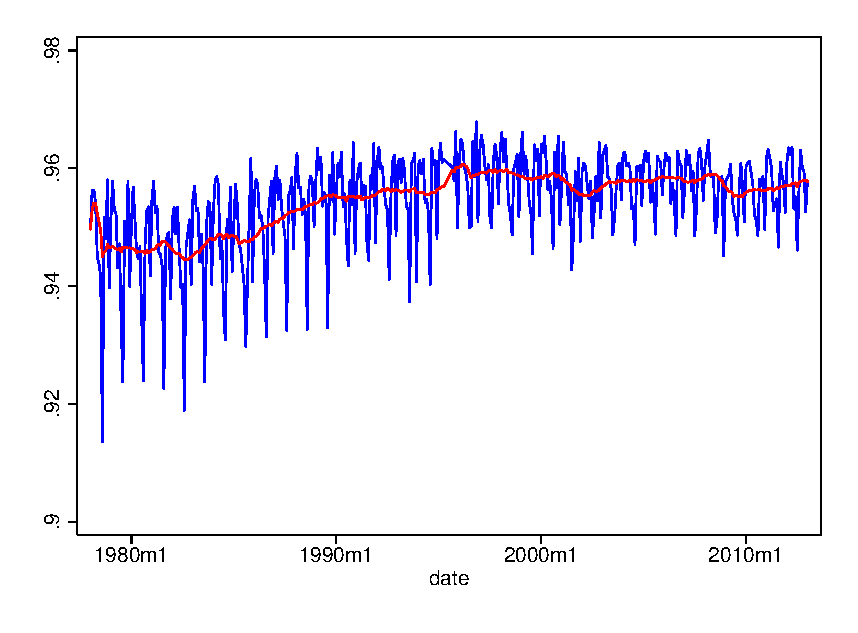
\includegraphics[width=.22\textwidth]{\results/EE.eps}}
    \subfloat[EU]{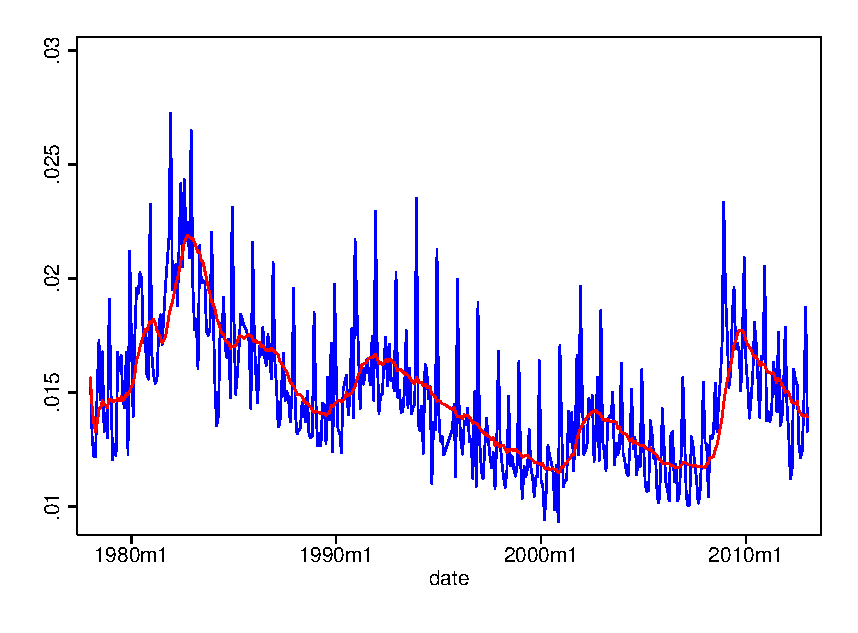
\includegraphics[width=.22\textwidth]{\results/EU.eps}}
    \subfloat[EN]{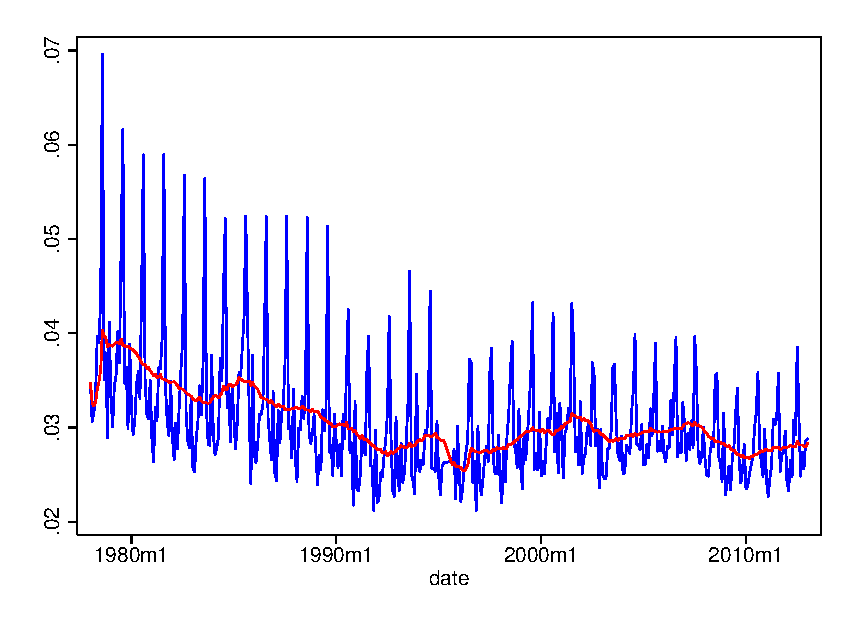
\includegraphics[width=.22\textwidth]{\results/EN.eps}}\\
    \subfloat[UE]{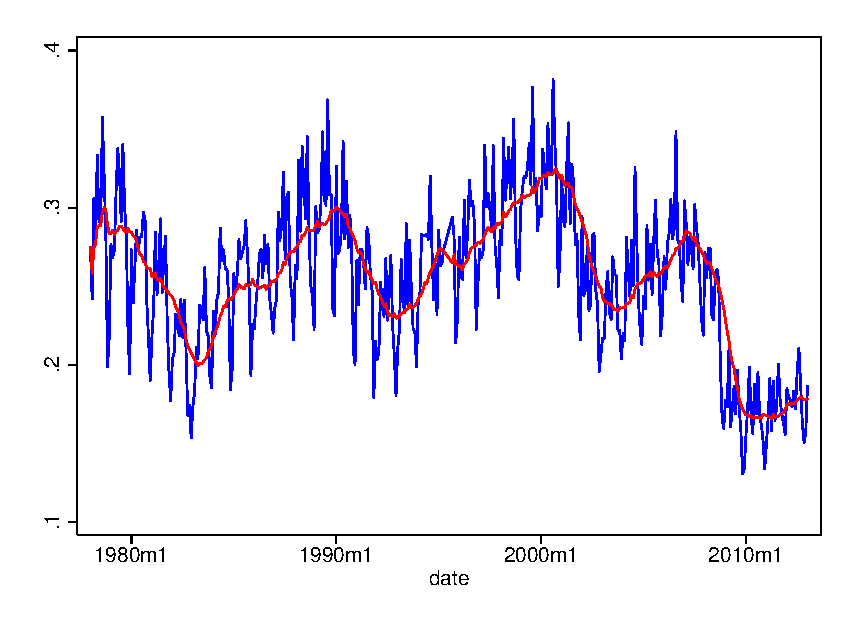
\includegraphics[width=.22\textwidth]{\results/UE.eps}}
    \subfloat[UU]{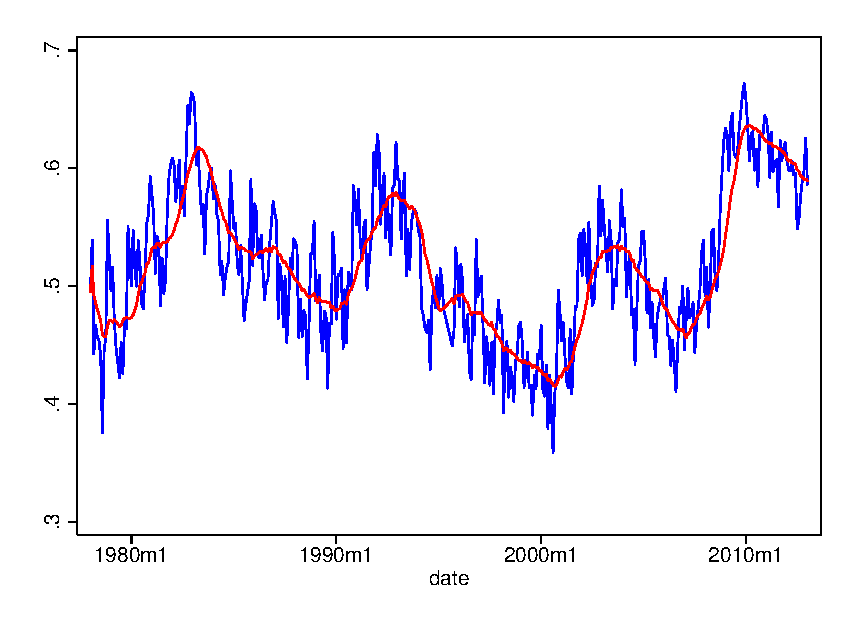
\includegraphics[width=.22\textwidth]{\results/UU.eps}}
    \subfloat[UN]{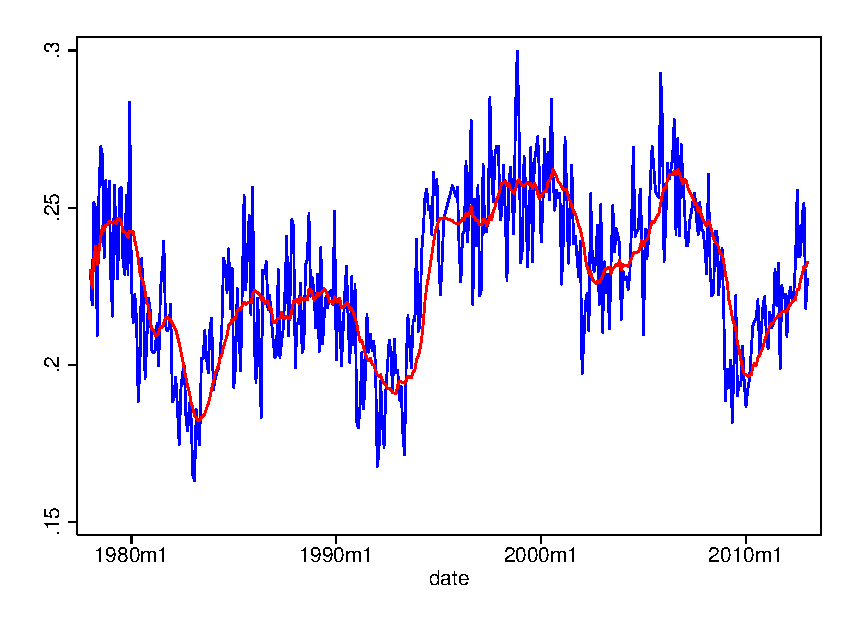
\includegraphics[width=.22\textwidth]{\results/UN.eps}}\\
    \subfloat[NE]{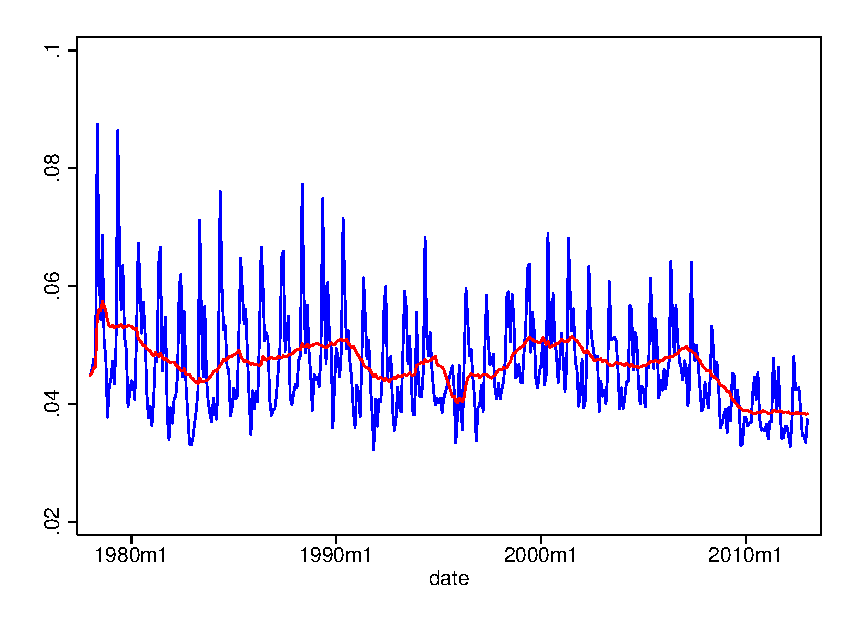
\includegraphics[width=.22\textwidth]{\results/NE.eps}}
    \subfloat[NU]{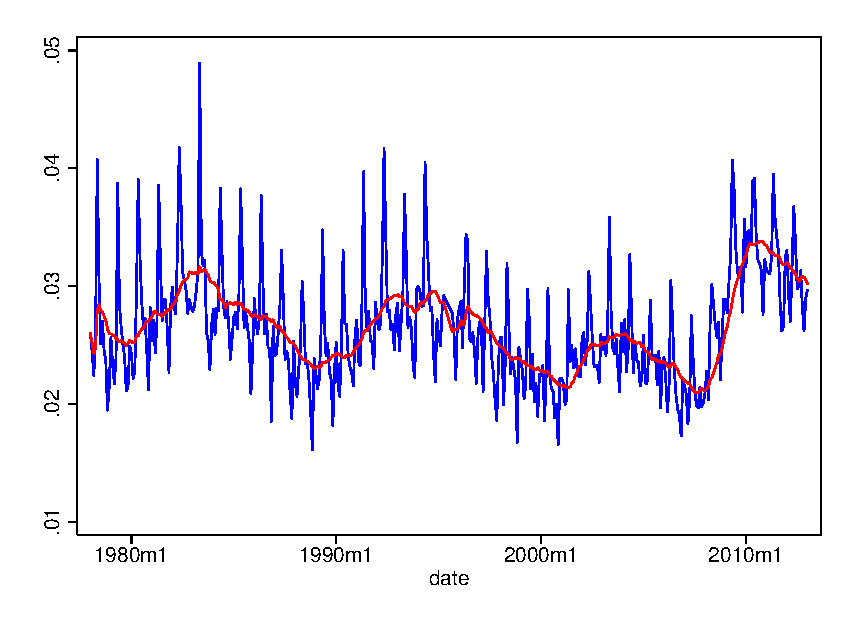
\includegraphics[width=.22\textwidth]{\results/NU.eps}}
    \subfloat[NN]{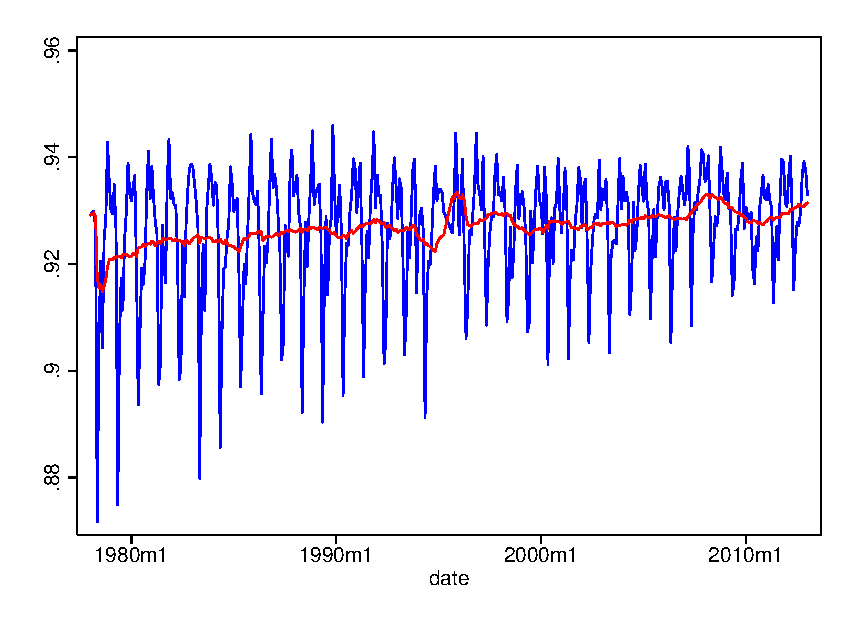
\includegraphics[width=.22\textwidth]{\results/NN.eps}}\\
    \flushleft \footnotesize Flows in blue; 12-month moving average in red.
    \flushleft \footnotesize Source: BLS and Author's Calculations
    \label{multipletable}
\end{figure}
    \end{lstlisting}
\end{frame}

\begin{frame}[fragile]{Combining multiple figures in Beamer}
    Unfortunately, Beamer does not support the \lst-subfig- package. You can still accomplish roughly the same task in Beamer, however, just without the subfigure captions.
    \begin{lstlisting}
\begin{figure}[h!]
    \caption{Labor Force Flows}
    \centering
    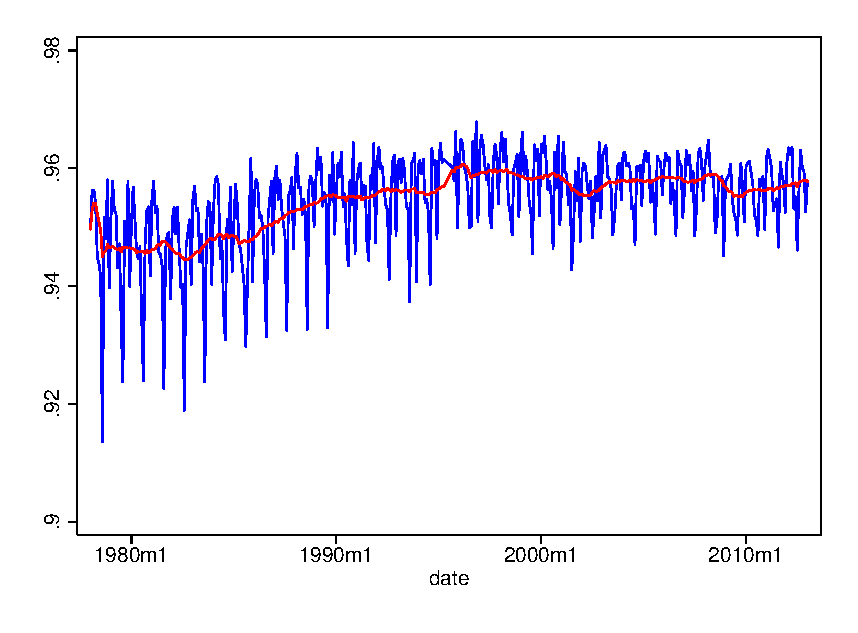
\includegraphics[width=.22\textwidth]{\results/EE.eps}
    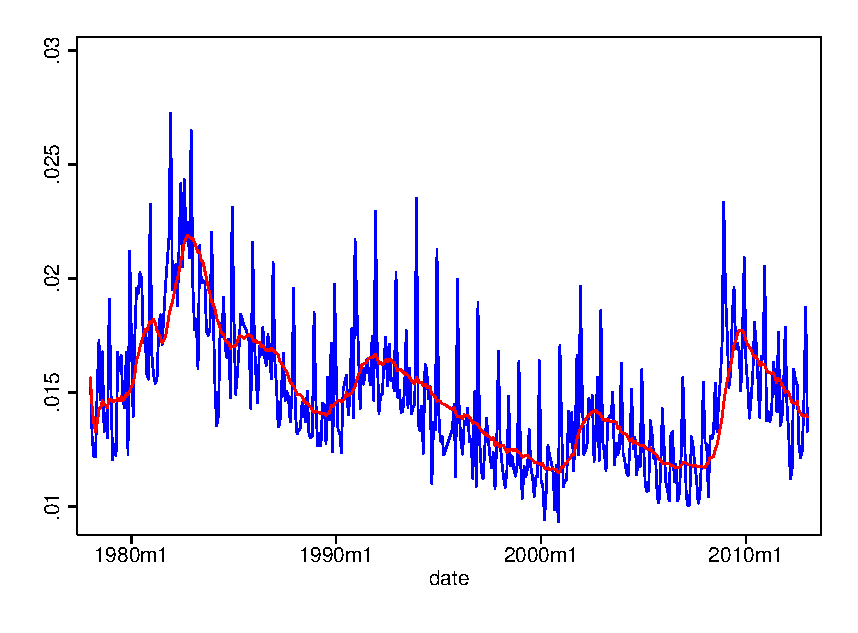
\includegraphics[width=.22\textwidth]{\results/EU.eps}
    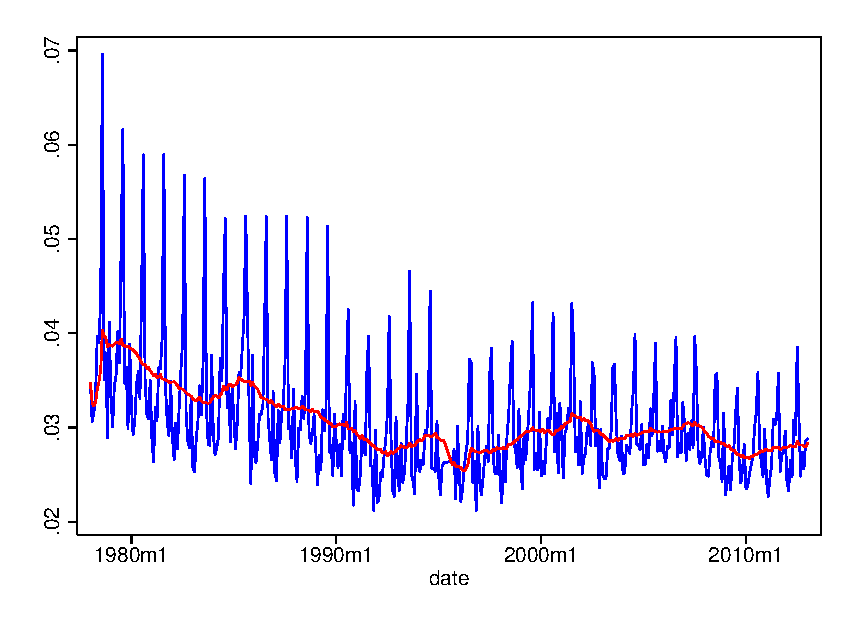
\includegraphics[width=.22\textwidth]{\results/EN.eps}\\
    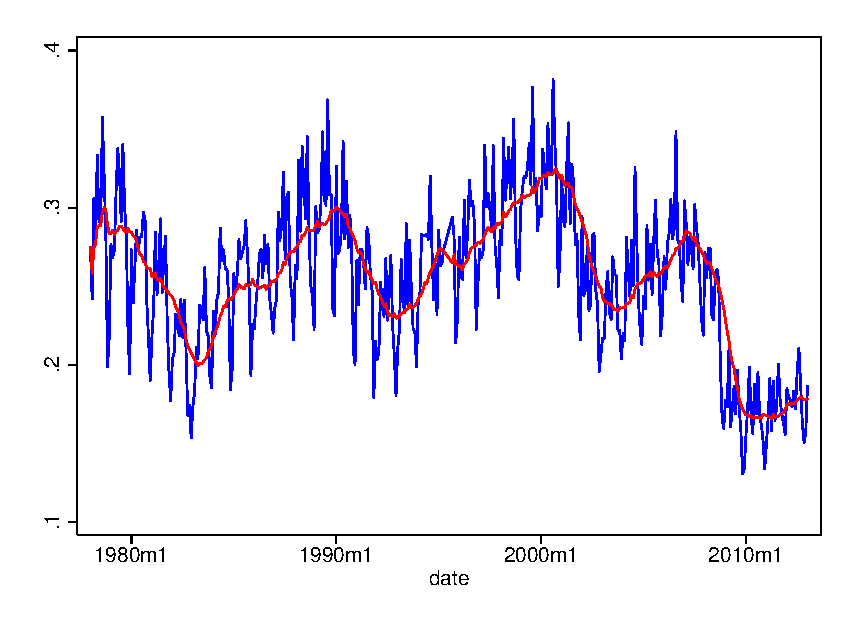
\includegraphics[width=.22\textwidth]{\results/UE.eps}
    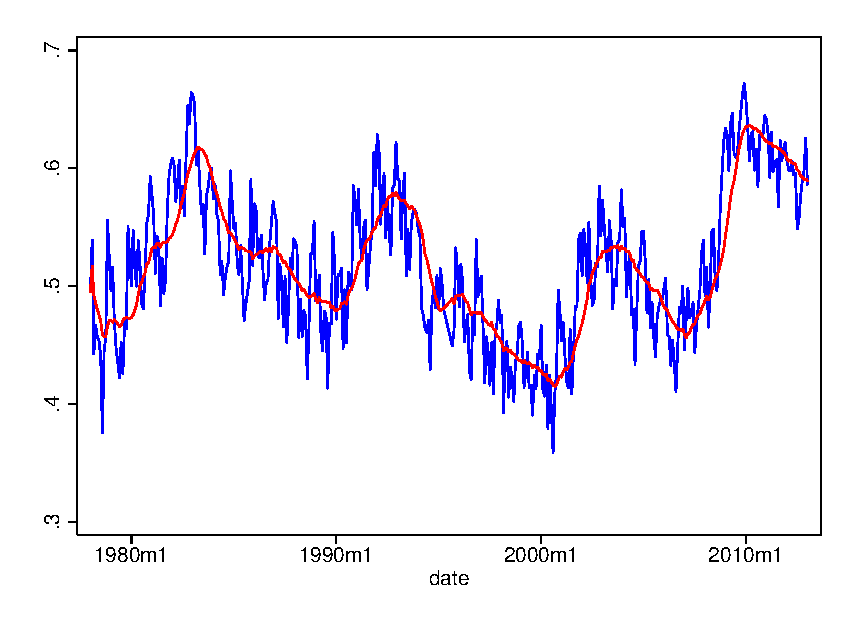
\includegraphics[width=.22\textwidth]{\results/UU.eps}
    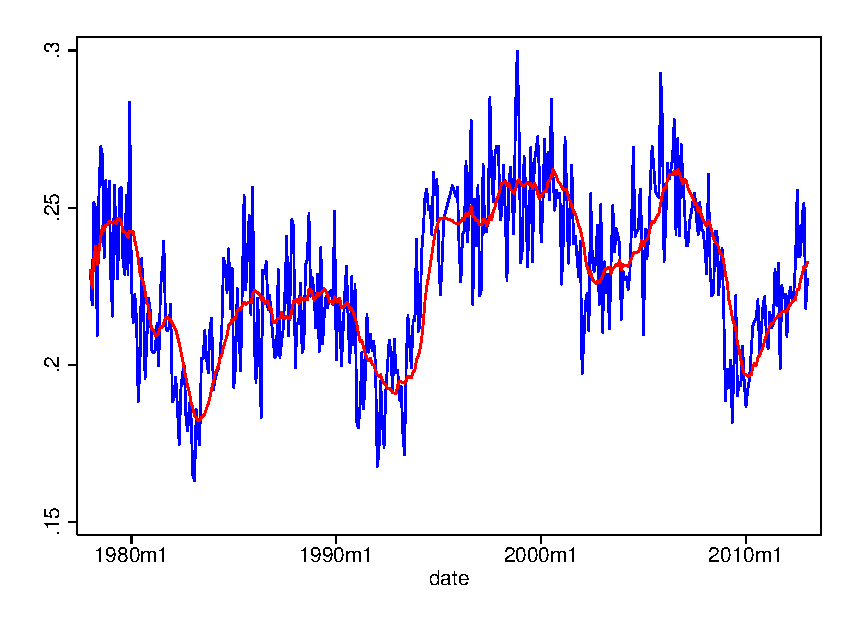
\includegraphics[width=.22\textwidth]{\results/UN.eps}\\
    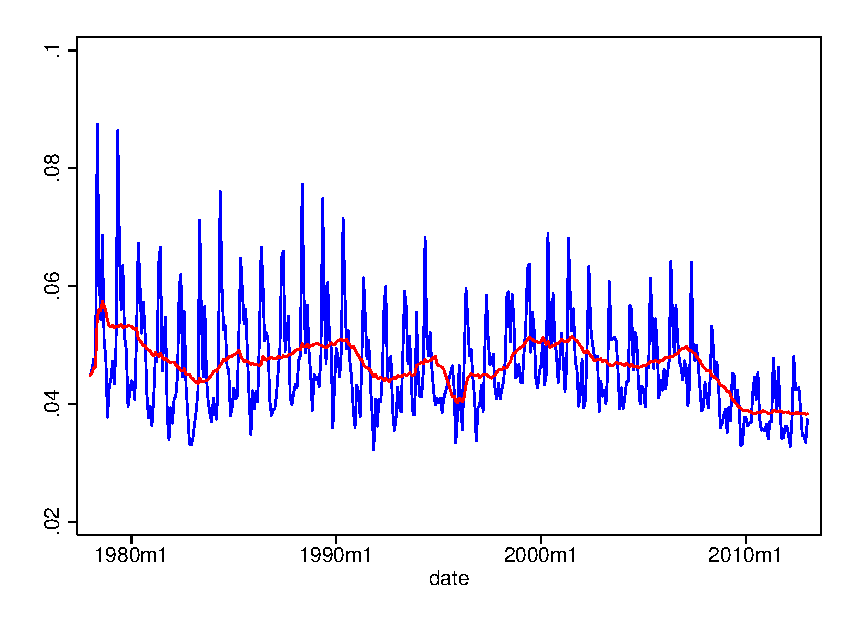
\includegraphics[width=.22\textwidth]{\results/NE.eps}
    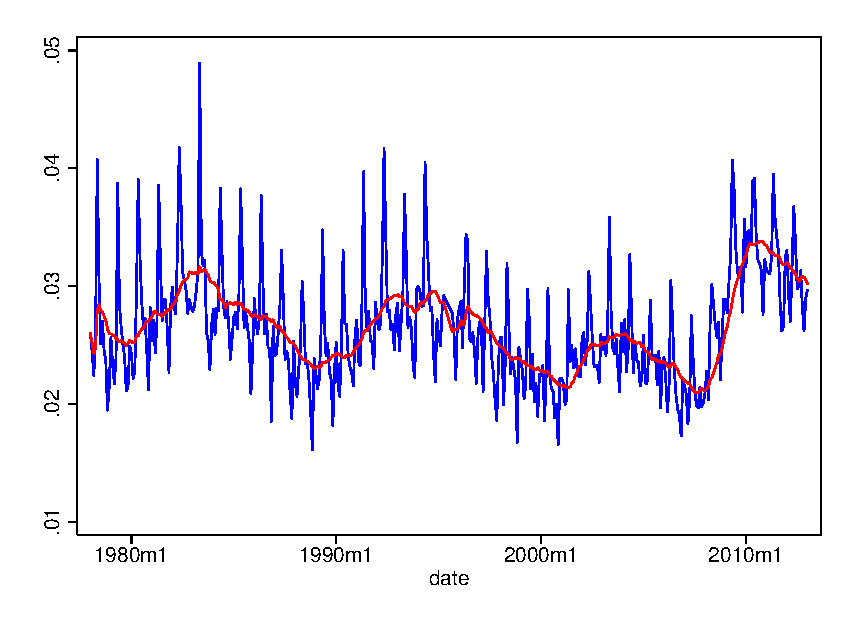
\includegraphics[width=.22\textwidth]{\results/NU.eps}
    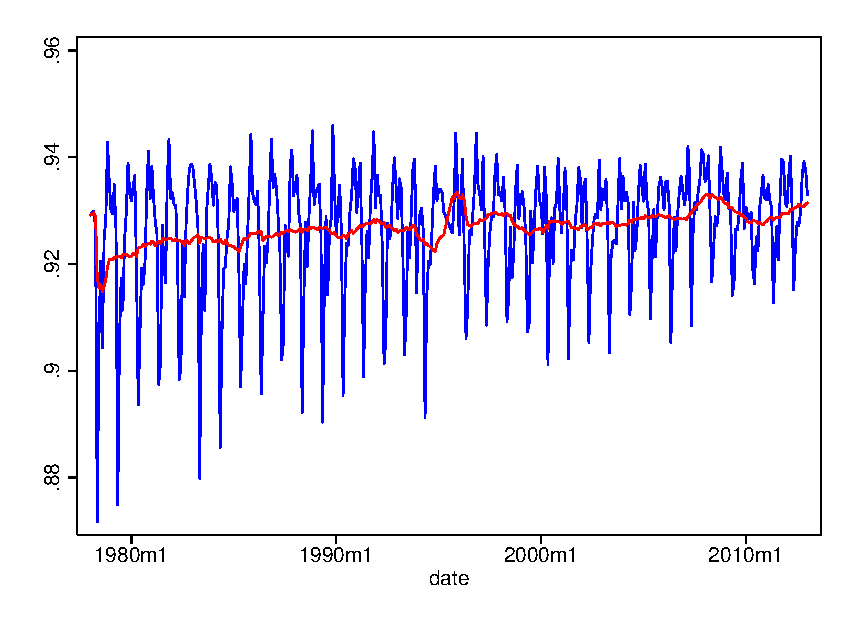
\includegraphics[width=.22\textwidth]{\results/NN.eps}\\
    \flushleft \footnotesize Flows in blue; 12-month moving average in red.
    \flushleft \footnotesize Source: BLS and Author's Calculations
    \label{multipletable}
\end{figure}
    \end{lstlisting}
\end{frame}

\begin{frame}[fragile]{Combining multiple figures in Beamer}
    \begin{figure}[h!]
        \caption{Labor Force Flows}
        \centering
        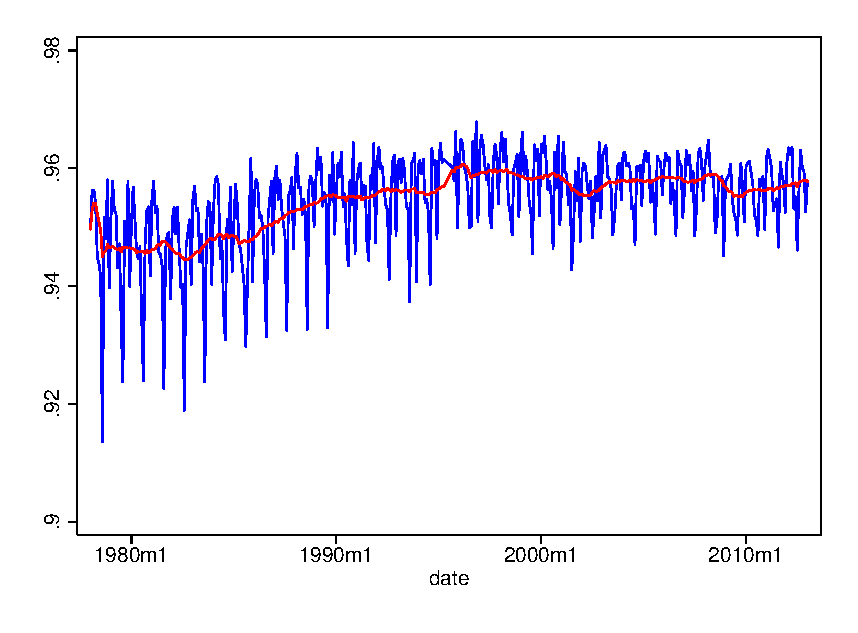
\includegraphics[width=.22\textwidth]{\results/EE.eps}
        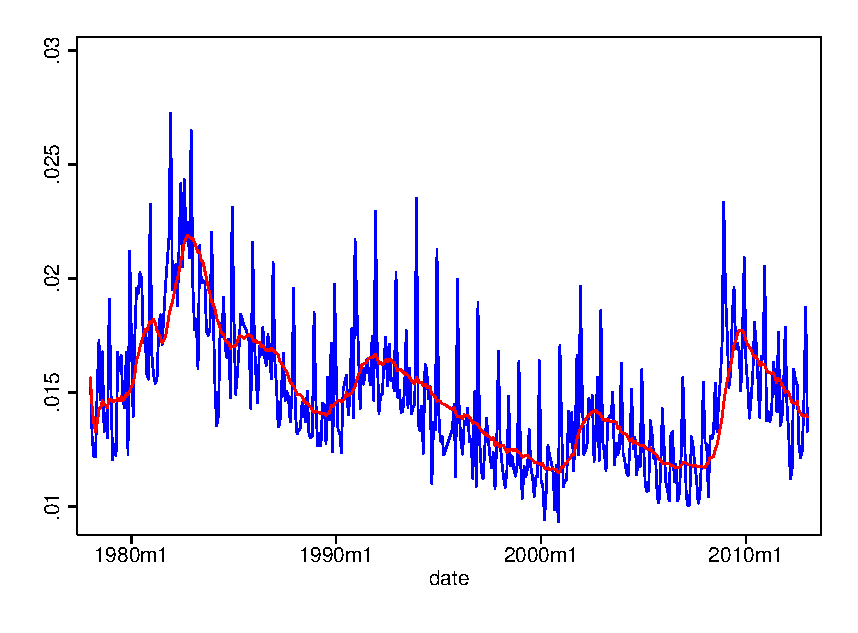
\includegraphics[width=.22\textwidth]{\results/EU.eps}
        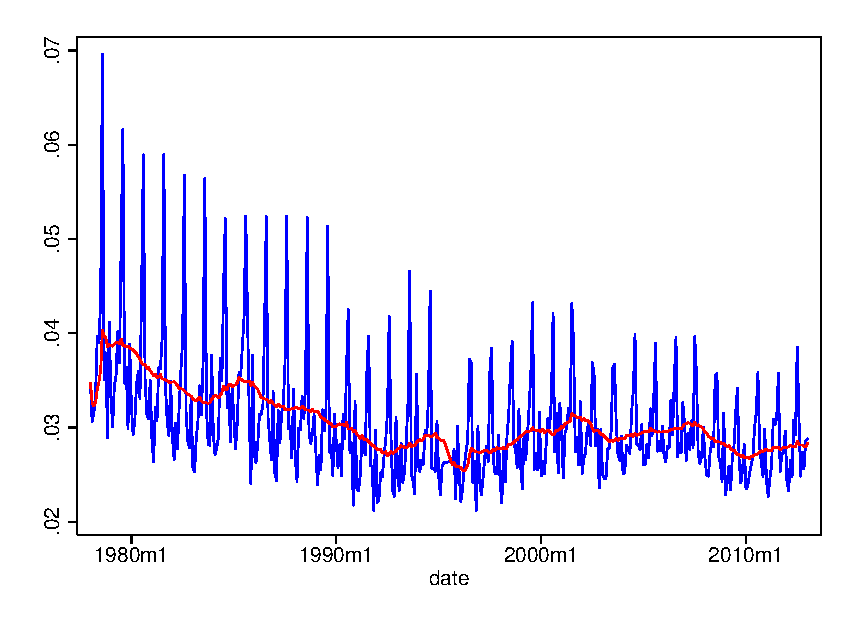
\includegraphics[width=.22\textwidth]{\results/EN.eps}\\
        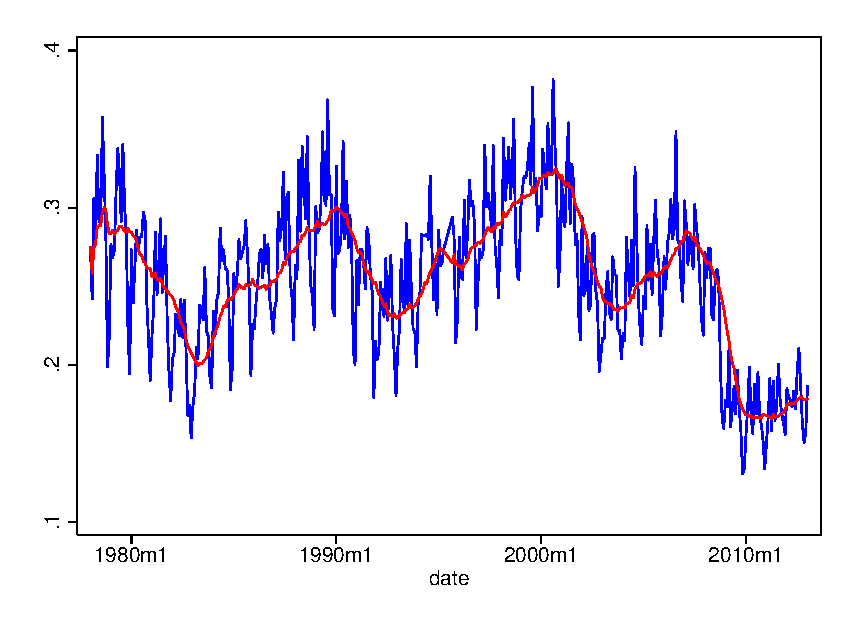
\includegraphics[width=.22\textwidth]{\results/UE.eps}
        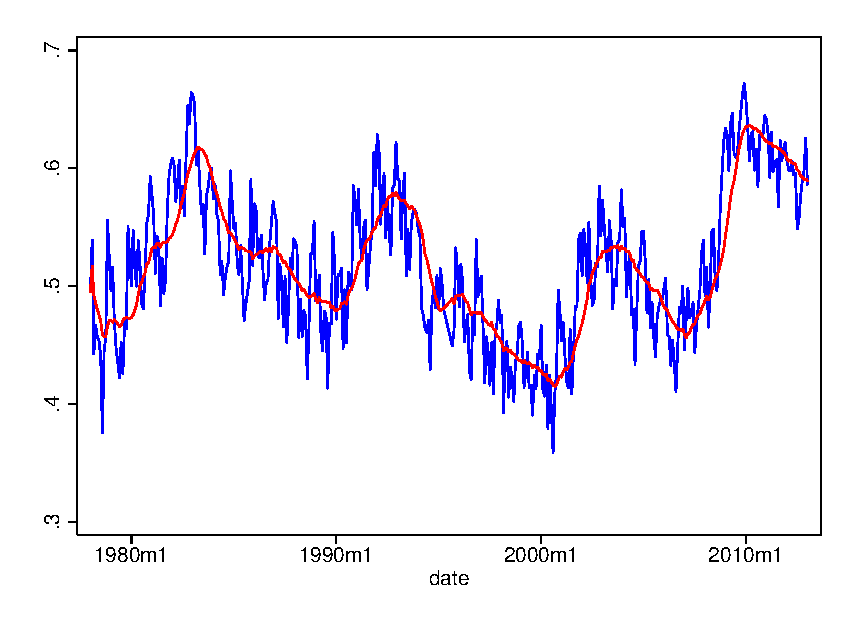
\includegraphics[width=.22\textwidth]{\results/UU.eps}
        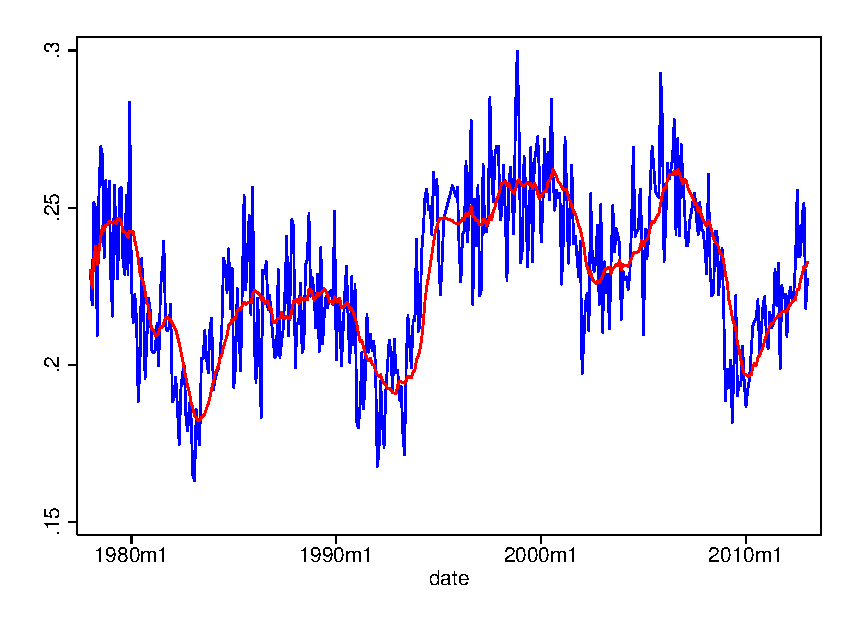
\includegraphics[width=.22\textwidth]{\results/UN.eps}\\
        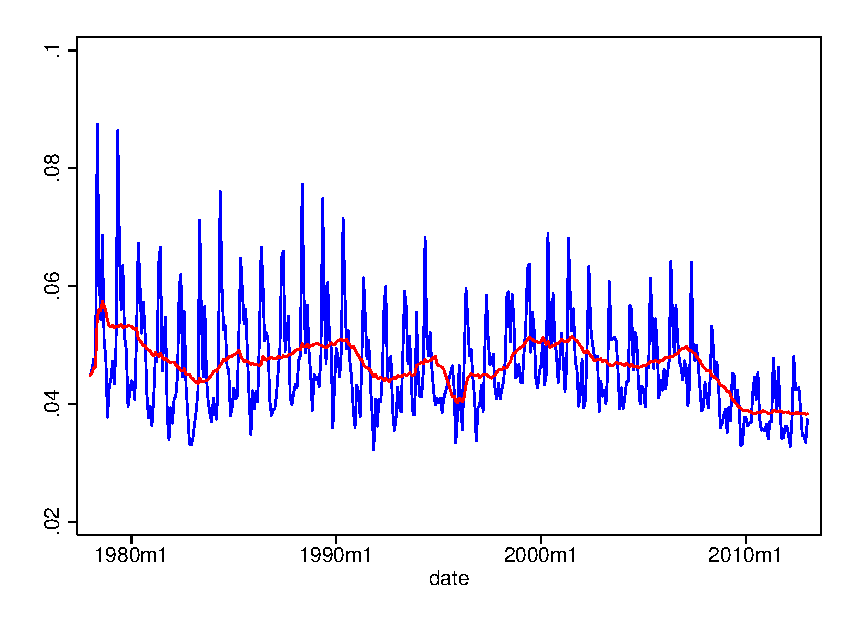
\includegraphics[width=.22\textwidth]{\results/NE.eps}
        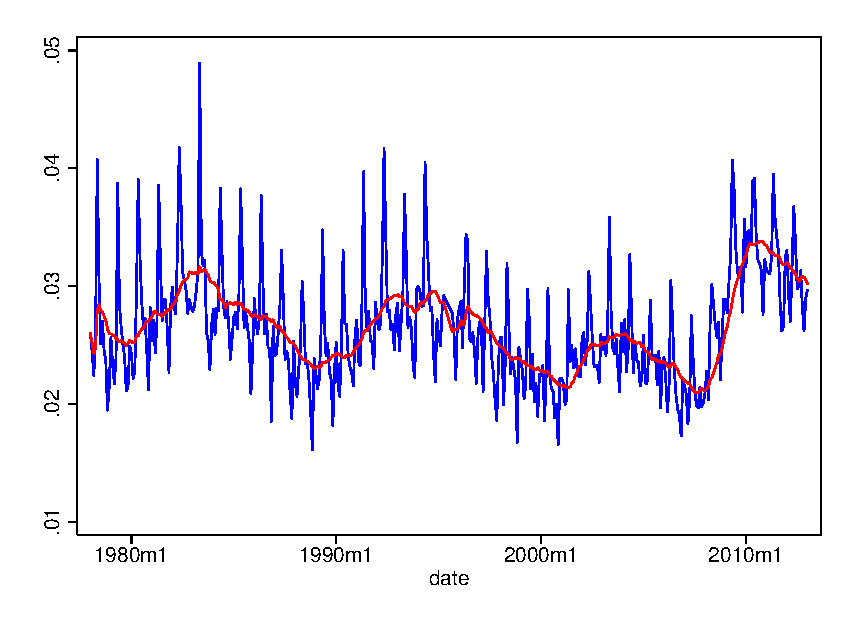
\includegraphics[width=.22\textwidth]{\results/NU.eps}
        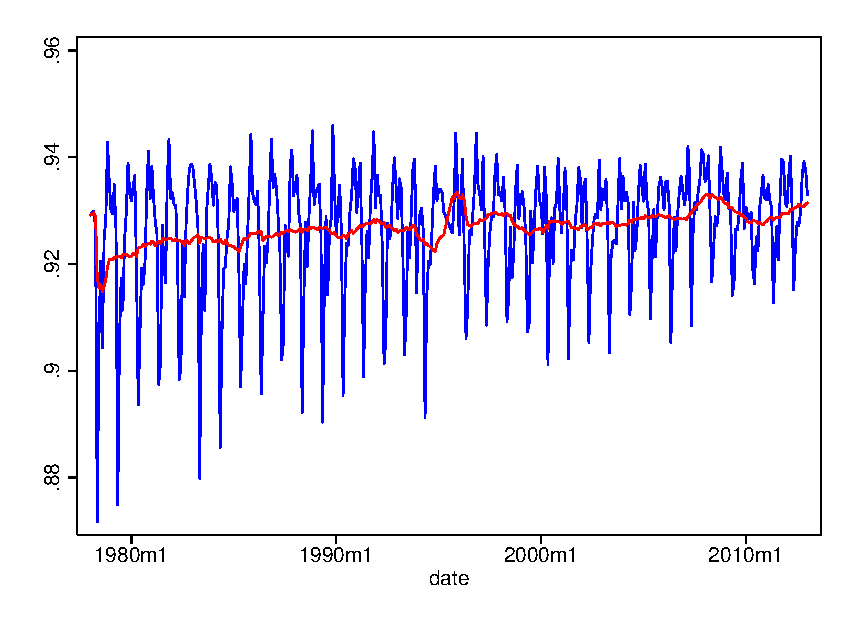
\includegraphics[width=.22\textwidth]{\results/NN.eps}\\
        \flushleft \footnotesize Flows in blue; 12-month moving average in red.
        \flushleft \footnotesize Source: BLS and Author's Calculations
        \label{multipletable}
    \end{figure}
\end{frame}

\begin{frame}[fragile]{Sideways Figures}
    Rotating a figure sideways is simple using the \lst=sidewaysfigure= environment instead of \lst=figure=. The below code reproduces the figure above but turns it sideways. You will notice that the only change I have made is changing \lst=begin{figure}= to \lst=begin{sidewaysfigure}= and \lst=end{figure}= to \lst=end{sidewaysfigure}=
        \begin{lstlisting}
\begin{figure}
    \caption{Labor Force Flows}
    \centering
    \subfloat[EE]{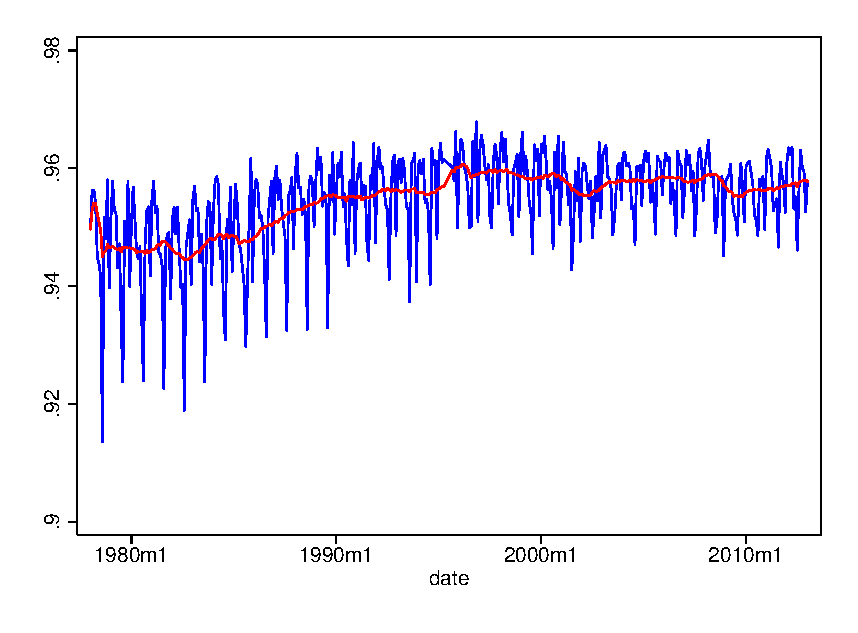
\includegraphics[width=.22\textwidth]{\results/EE.eps}}
    \subfloat[EU]{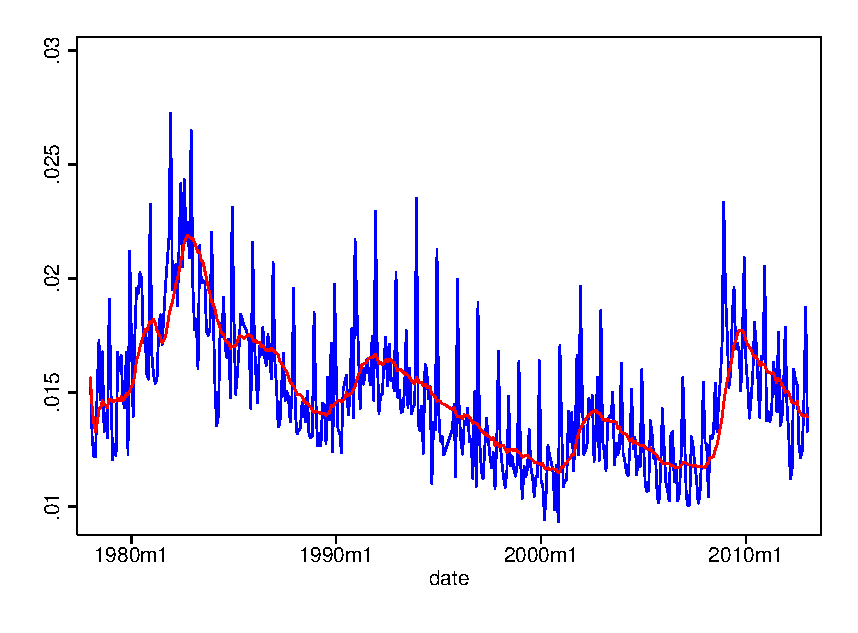
\includegraphics[width=.22\textwidth]{\results/EU.eps}}
    \subfloat[EN]{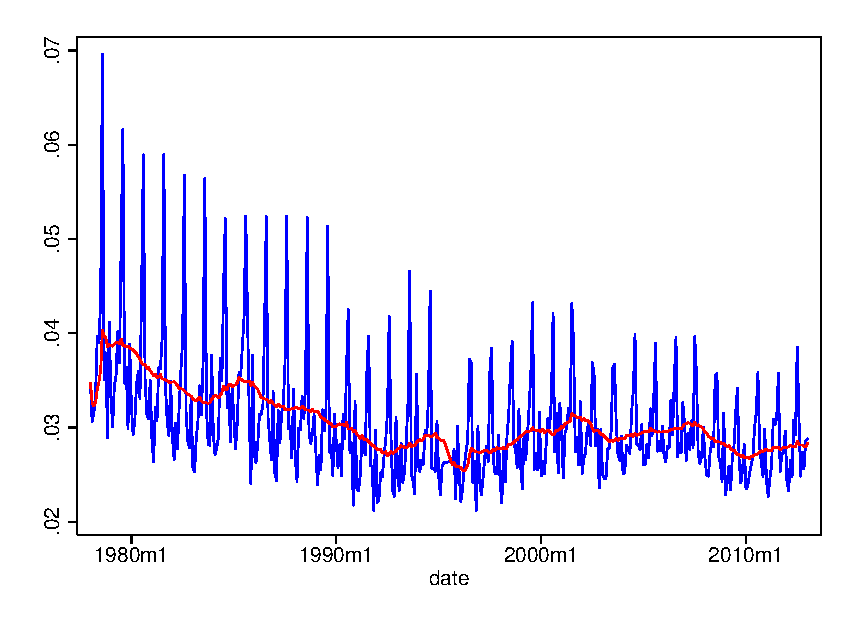
\includegraphics[width=.22\textwidth]{\results/EN.eps}}\\
    \subfloat[UE]{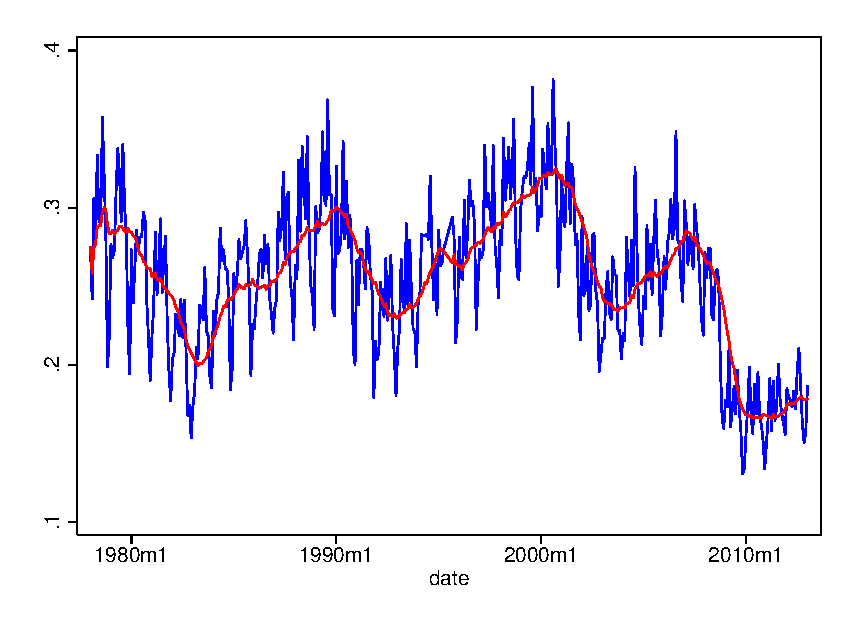
\includegraphics[width=.22\textwidth]{\results/UE.eps}}
    \subfloat[UU]{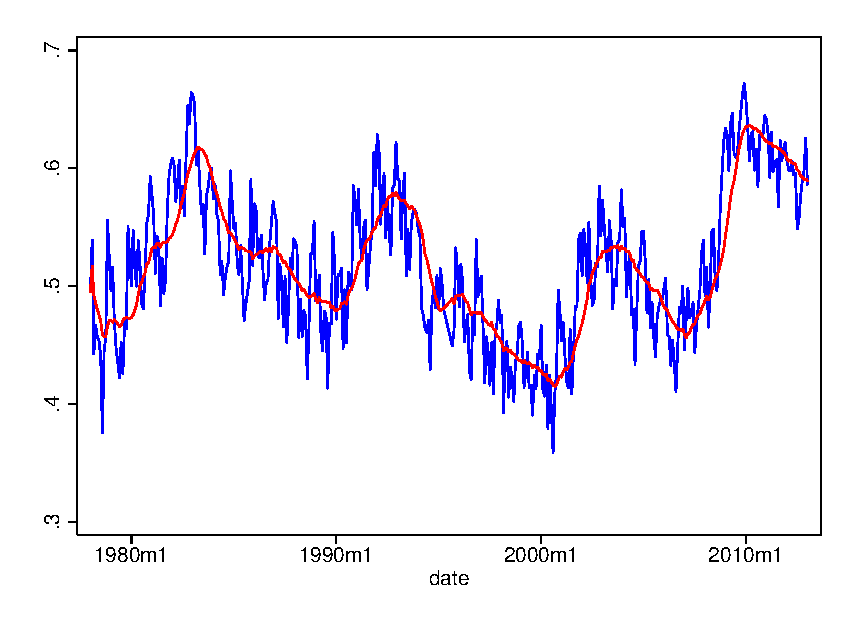
\includegraphics[width=.22\textwidth]{\results/UU.eps}}
    \subfloat[UN]{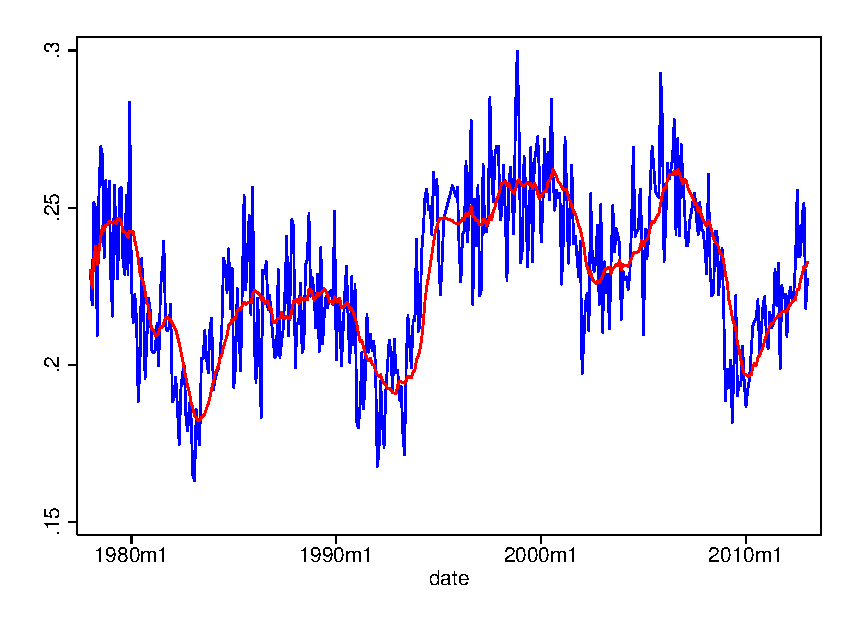
\includegraphics[width=.22\textwidth]{\results/UN.eps}}\\
    \subfloat[NE]{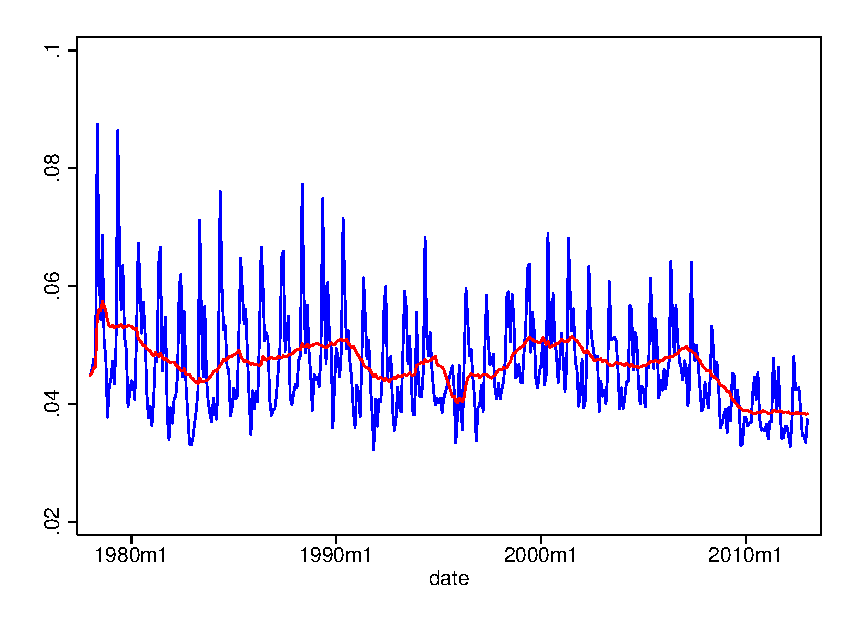
\includegraphics[width=.22\textwidth]{\results/NE.eps}}
    \subfloat[NU]{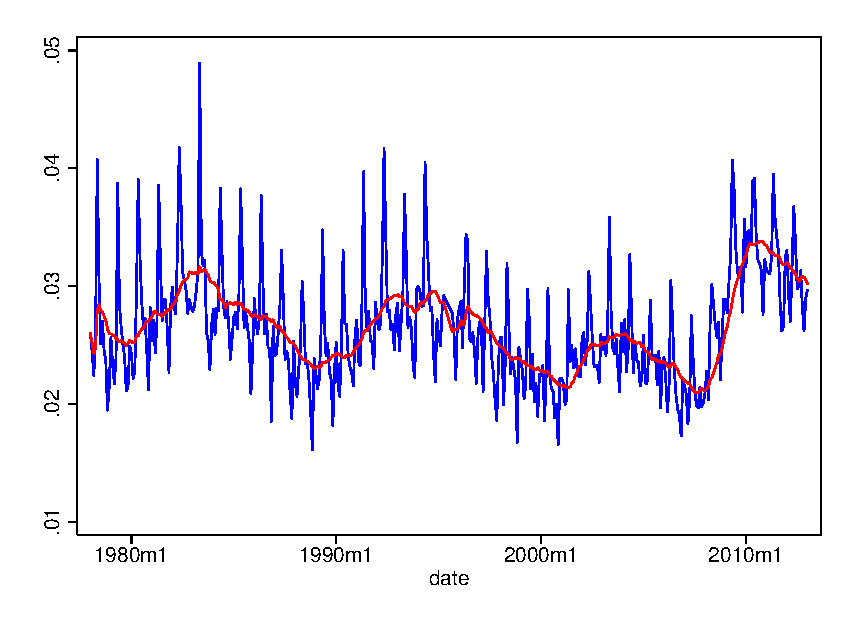
\includegraphics[width=.22\textwidth]{\results/NU.eps}}
    \subfloat[NN]{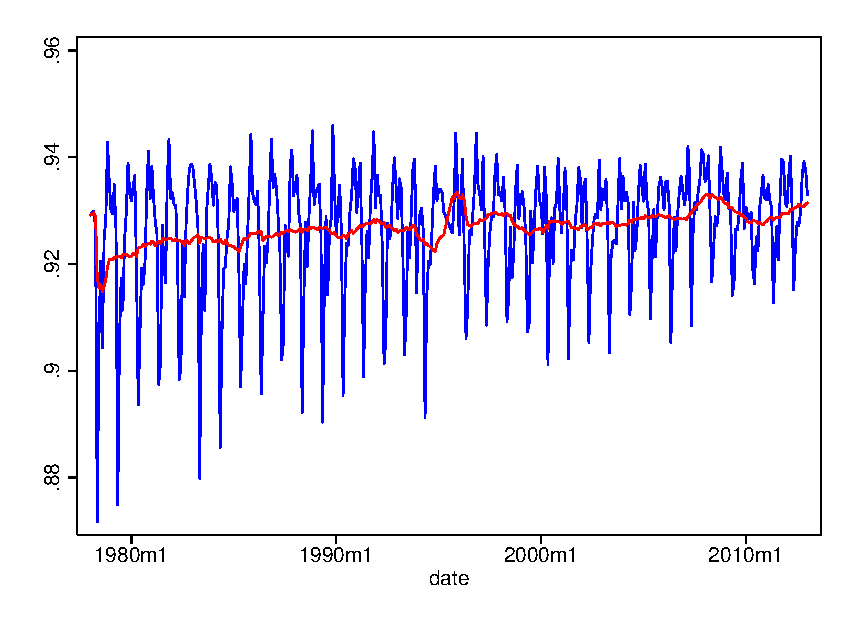
\includegraphics[width=.22\textwidth]{\results/NN.eps}}\\
    \flushleft \footnotesize Flows in blue; 12-month moving average in red.
    \flushleft \footnotesize Source: BLS and Author's Calculations
    \label{multipletable}
\end{figure}
    \end{lstlisting}
\end{frame}

\section{Tables}

\begin{frame}[fragile]{How do I create a table in \LaTeX{}?}
    There are three environments you should be familiar with as you learn to use \LaTeX{} --- \lst=tabular=, \lst=table=, and \lst=longtable=.
    \begin{enumerate}
        \item \lst=tabular= --- The \lst=tabular= environment creates the table itself (i.e. columns, lines, etc).
        \item \lst=table= --- The \lst=table= environment contains a \lst=tabular= and controls the location of the table within the document and allows you to add captions and labels.
        \item \lst=longtable= --- The \lst=longtable= environment combines the functionality of both the \lst=table= and \lst=tabular= environments and allows tables to continue for more than one page.
    \end{enumerate}
\end{frame}

\subsection{The Tabular Environment}

\begin{frame}[fragile]{The Tabular Environment}
    \begin{itemize}
        \item The \lst==tabular= environment is opened by \lst+\begin{tabular}{specs}+ and ends with \lst+\end{tabular}+, where \emph{specs} defines how many columns the table will have and how they should be aligned.
        \item \LaTeX{}'s \lst==tabular= environment has a number of commands that control the look of your table, but the two most important are \verb+&+ and \verb+\\+. The \verb+&+ command  delimits cells within a table and \verb+\\+ ends a line.
    \end{itemize}
    The below table, therefore, has one left-aligned column followed by two right-aligned columns: \\
    \vspace{.5cm}
    \pause
    \begin{columns}[t]
        \column{.5\textwidth}
            \vspace{-1.5cm}
            \begin{lstlisting}
\begin{tabular}{lrr}
    Car type&No.&\% \\
    \midrule
    Domestic&52.0&70.3 \\
    Foreign&22.0&29.7 \\
    Total&74.0&100.0 \\
\end{tabular}
            \end{lstlisting} \pause
        \column{.5\textwidth}
            \begin{tabular}{lrr}
                Car type&No.&\% \\
                \midrule
                Domestic&52.0&70.3 \\
                Foreign&22.0&29.7 \\
                Total&74.0&100.0 \\
            \end{tabular}
    \end{columns}
\end{frame}

\subsection{The Table Environment}

\begin{frame}[fragile]{The Table Environment}
    Enclosing your \lst=tabular= within a \lst=table= allows you to include a caption and/or a label and provides greater control over the location of your table within the document. This is especially useful if you would like to include a table of contents and hyperlinks. \pause

    \begin{columns}[t]
        \column{.5\textwidth}
        \begin{lstlisting}
\begin{table}
    \caption{Origin of Cars}
    \label{mytablelabel}
    \begin{tabular}{lrr}
        Car type&No.&\% \\
        \midrule
        Domestic&52.0&70.3 \\
        Foreign&22.0&29.7 \\
        Total&74.0&100.0 \\
    \end{tabular}
    \footnotesize My footnote...
\end{table}
    \end{lstlisting} \pause
        \column{.5\textwidth}
        \begin{table}
            \caption{Origin of Cars}
            \label{mytablelabel}
            \begin{tabular}{lrr}
                Car type&No.&\% \\
                \midrule
                Domestic&52.0&70.3 \\
                Foreign&22.0&29.7 \\
                Total&74.0&100.0 \\
            \end{tabular}\\
            \footnotesize My footnote...
        \end{table}
    \end{columns}
\end{frame}

\subsection{The Longtable Environment}

\begin{frame}[fragile]{The Longtable Environment}
    The \lst=longtable= environment combines the table creation of \lst=tabular= with \lst=table='s ability to create captions, footnotes, etc. More importantly, \lst=longtable= allows you create tables that span multiple pages (only in length, not width, unfortunately). This doesn't really work in Beamer so I won't provide a nice example, but \lst=longtable= will very likely come in handy when you are presenting results of a regression with many independent variables. \pause

    \begin{columns}[t]
        \column{.5\textwidth}
    \begin{lstlisting}
\begin{longtable}{lrr}
    \caption{Origin of Cars} \\
    \label{mytablelabel} \\
        Car type&No.&\% \\
        \midrule
        Domestic&52.0&70.3 \\
        Foreign&22.0&29.7 \\
        Total&74.0&100.0 \\
    \footnotesize My footnote...
\end{longtable}
    \end{lstlisting} \pause
        \column{.5\textwidth}
        \begin{longtable}{lrr}
            \caption{Origin of Cars}\\
            \label{mytablelabel}\\
                Car type&No.&\% \\
                \midrule
                Domestic&52.0&70.3 \\
                Foreign&22.0&29.7 \\
                Total&74.0&100.0 \\
            \footnotesize My footnote...
        \end{longtable}
    \end{columns}
\end{frame}



\section{Hyperlinks}

\begin{frame}[fragile]
    \LaTeX{} enables users to easily add hyperlinks to their documents.
    \begin{itemize}
        \item \url{http://en.wikibooks.org/wiki/LaTeX/Hyperlinks} is a great source for more information on hyperlinks \pause
        \item Including the whole url in the text can be a bit clunky, however, so you may want to add a description to the link. The same website can be accessed by \href{http://en.wikibooks.org/wiki/LaTeX/Hyperlinks}{clicking here}. \pause
        \item You can insert email links. You can email me by \href{mailto:james.fogel@bos.frb.org}{clicking here} or clicking on my email address, \href{mailto:james.fogel@bos.frb.org}{james.fogel@bos.frb.org}. \pause
        \item  All the links you see here are highlighted in blue, however you can change the color by editing the \lst=\hypersetup{ ... }= command in the document preamble or anywhere else in the document. For example, I can change the email link to green\hypersetup{urlcolor=green}: \href{mailto:james.fogel@bos.frb.org}{james.fogel@bos.frb.org}; or black: \hypersetup{urlcolor=black} \href{mailto:james.fogel@bos.frb.org}{james.fogel@bos.frb.org}.
    \end{itemize}
\end{frame}

\section{BibTeX}

\begin{frame}{BibTeX}
    BibTeX is \LaTeX{}'s bibliographic management tool. Rather than go into it here I will direct you to the data wiki, where Rich Ryan and Zack Kimball put together an excellent guide to BibTeX: \url{https://wiki.glc.frb.org/display/BOSRES/BibTeX}
\end{frame}

\section{Some Common Errors You Will Encounter at Compilation}

\begin{frame}[fragile]
    Wikibooks has a section explaining some of the more common errors that prevent your document from compiling: \url{http://en.wikibooks.org/wiki/LaTeX/Errors_and_Warnings.}

    Some others:
    \begin{itemize}
        \item \lst= ! Extra alignment tab has been changed to \cr = --- You specified the wrong number of columns in a tabular environment
        \item \lst= ! File ended while scanning use of \@writefile.= 
              \lst= <inserted text> \par ... \begin{ document} = --- Delete the .aux file in the directory where your .tex file is saved. This sometimes occurs after compilation failed on the previous attempt.
    \end{itemize}
\end{frame}

\section{Where to Go For Help}

\begin{frame}{Where to go for help}
    \begin{enumerate}
        \item Wikibooks offers an excellent source for \LaTeX{} knowledge. I recommend visiting this site first, especially early on while you are still trying to master the more basic tasks: \url{http://en.wikibooks.org/wiki/LaTeX}
        \item Ask me or another RA for help. There is a good chance I will be able to send you a snippet of code to accomplish your task
        \item Google
    \end{enumerate}
\end{frame}

\end{document}






